\section{Application and Experiments}

\begin{frame}[fragile, t]{Application and Experiments}
  \begin{block}{Space-Time Kernel Density Estimation}<1->
    \[ f(x, t) = \frac{1}{nh} \sum_{i=1}^{n} K\left(\frac{x - x_i}{h}, \frac{t - t_i}{h_t}\right) \]
    \begin{itemize}
      \item Parallelized summation leads to race condition.
      \item Implementation of space-time decomposition by Hohl et. al. \cite{kernel_estimation_1}.
      \item Parallelization by exploiting symmetry by Saule et. al. \cite{kernel_estimation_2}.
    \end{itemize}
  \end{block}

  \begin{block}{Authors Approach}<2->
    \begin{itemize}
      \item<3-> Arbitrary decomposition of space-time domain.
      \item<4-> 2 spatial coordinates, 1 time coordinate $\mapsto$ 3DS-IVC Problem
      \item<5-> number of datapoints within one voxel is set as weight.\footnotemark
      \item<5-> Weight $\propto$ computational costs.
    \end{itemize}
  \end{block}

  \vspace{0pt}
  \only<5->{
    \footnotetext{Voxel is the 3D equivalent of a Pixel}
  }
\end{frame}


\begin{frame}{Performance Profiles and Elapsed Time}
  \begin{figure}
    \begin{subfigure}{0.4\textwidth}
      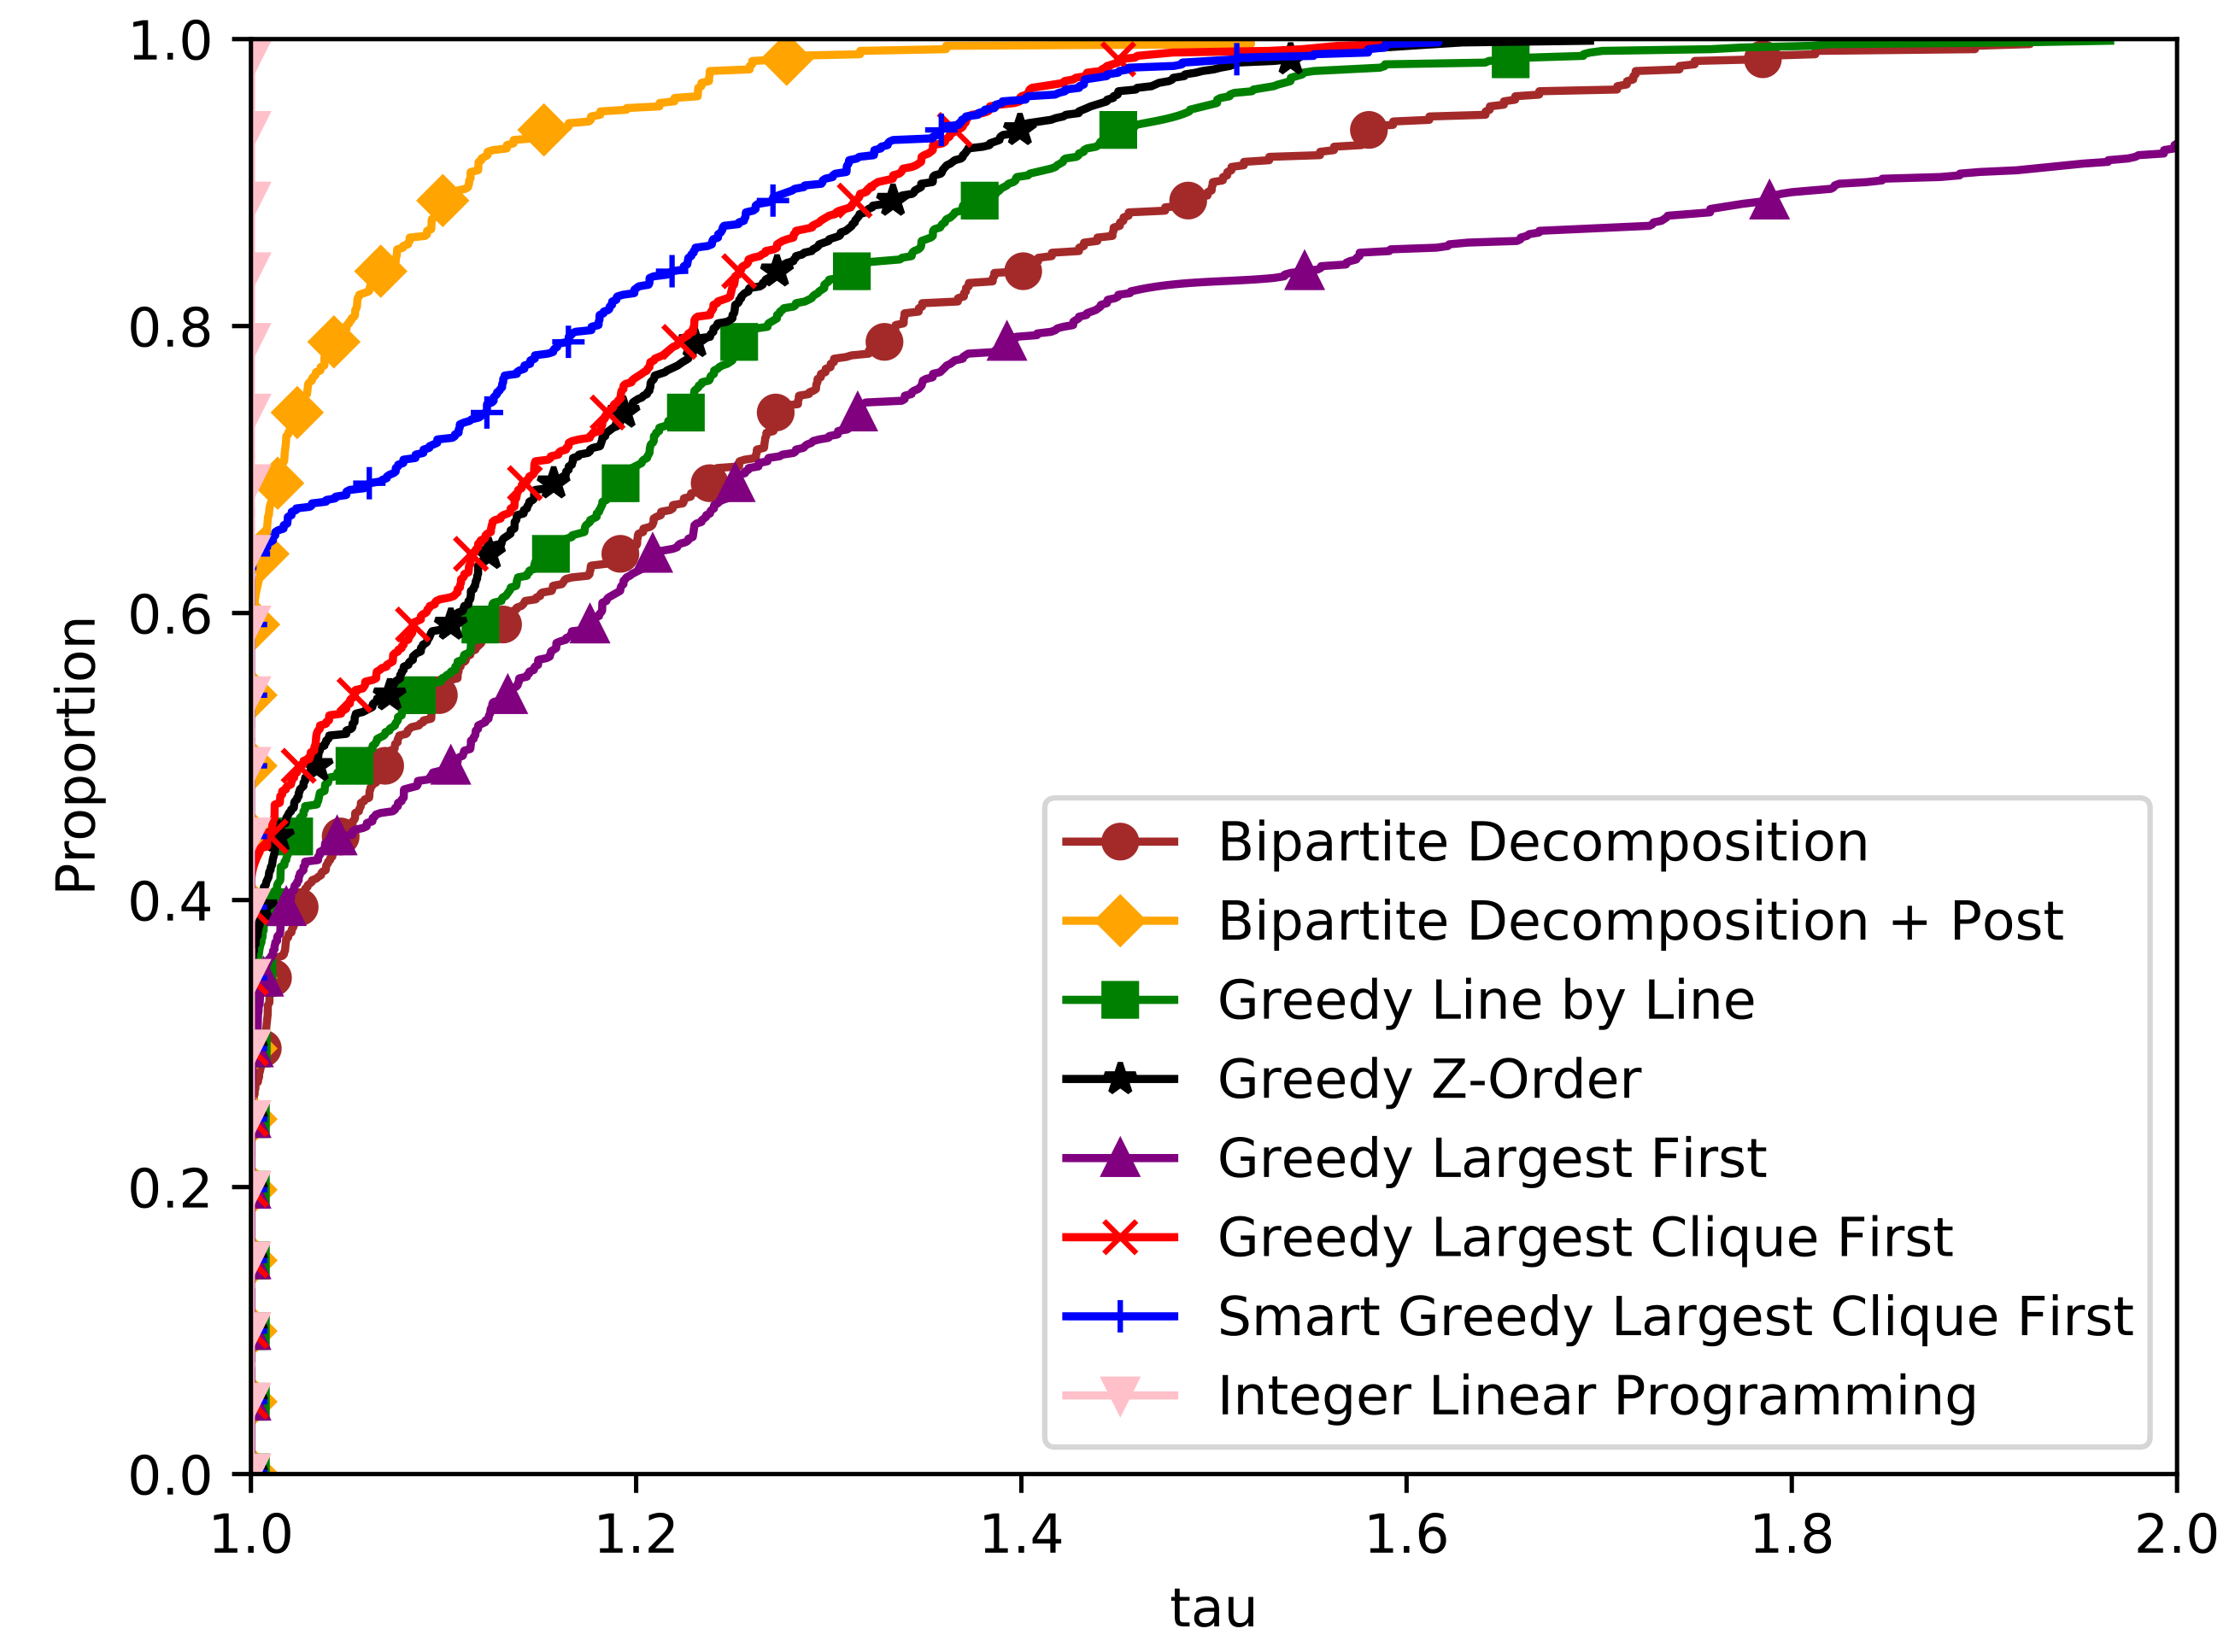
\includegraphics[width=\linewidth]{figures/2d_results_ilp.png}
      \caption{2D Instances. \footnotemark[1]}
    \end{subfigure}
    \hfill
    \begin{subfigure}{0.4\textwidth}
      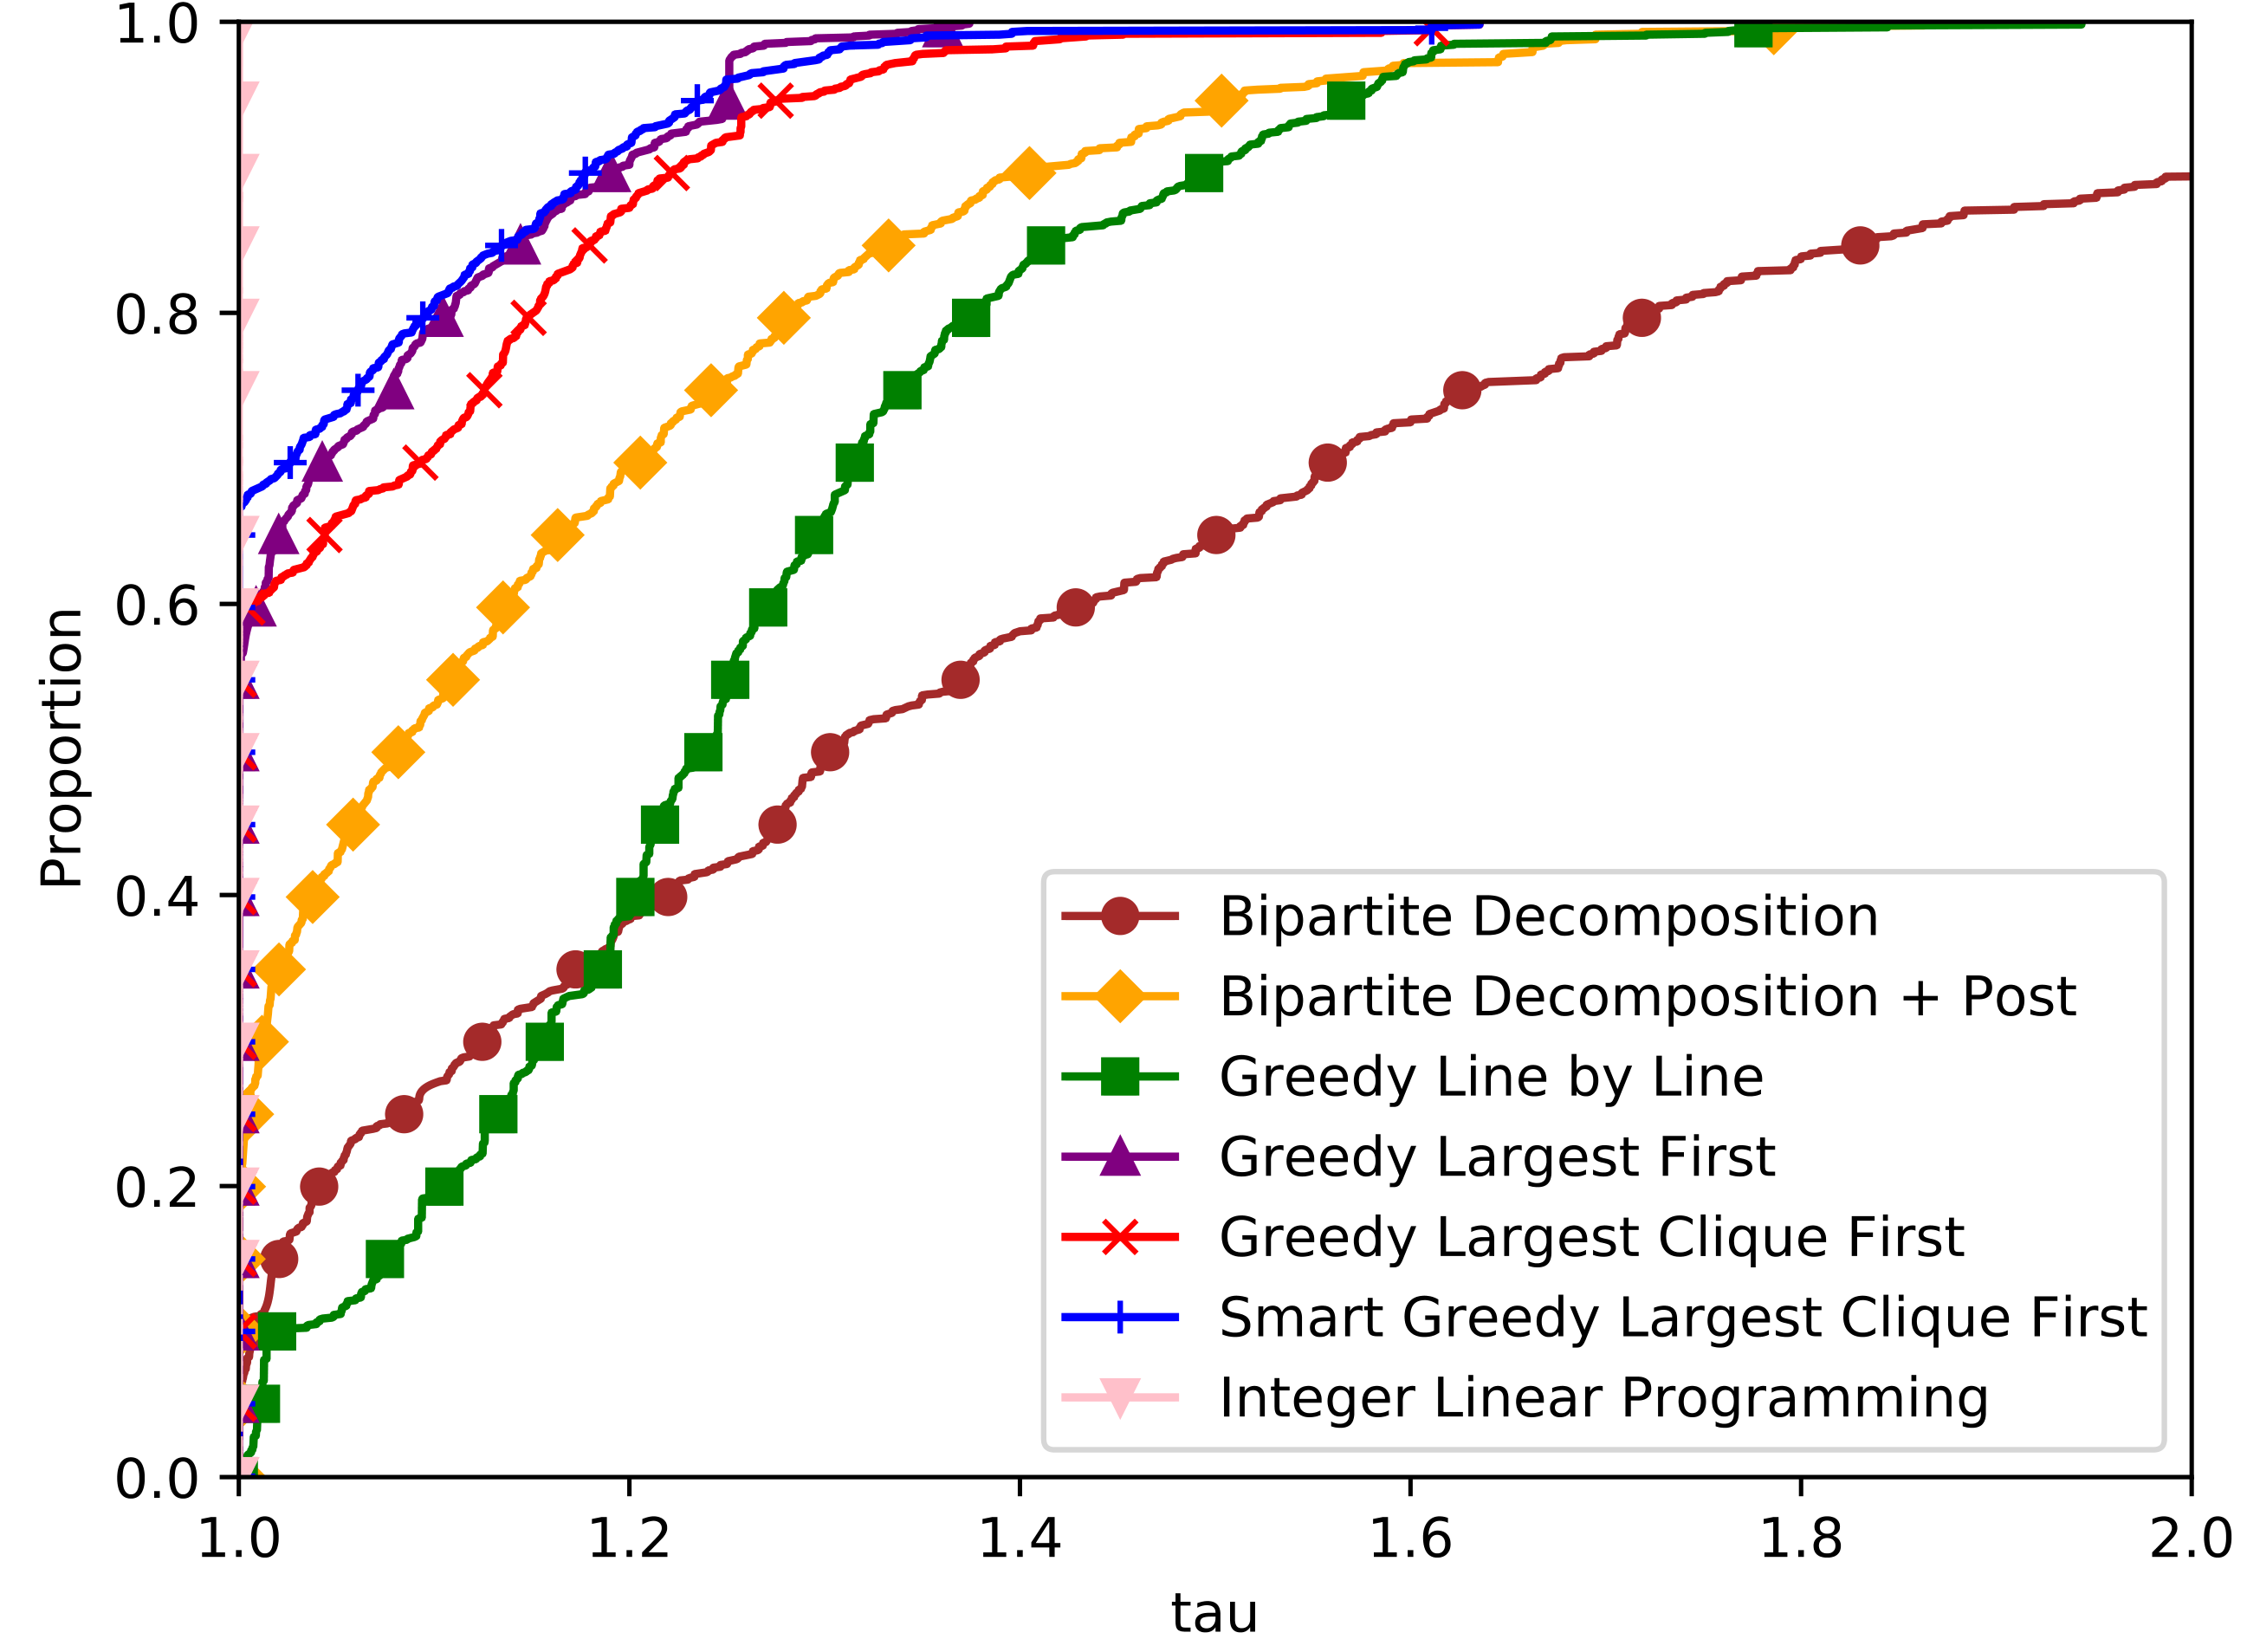
\includegraphics[width=\linewidth]{figures/3d_results_ilp.png}
      \caption{3D Instances. \footnotemark[1]}
    \end{subfigure}

    \medskip

    \begin{subfigure}{0.4\textwidth}
      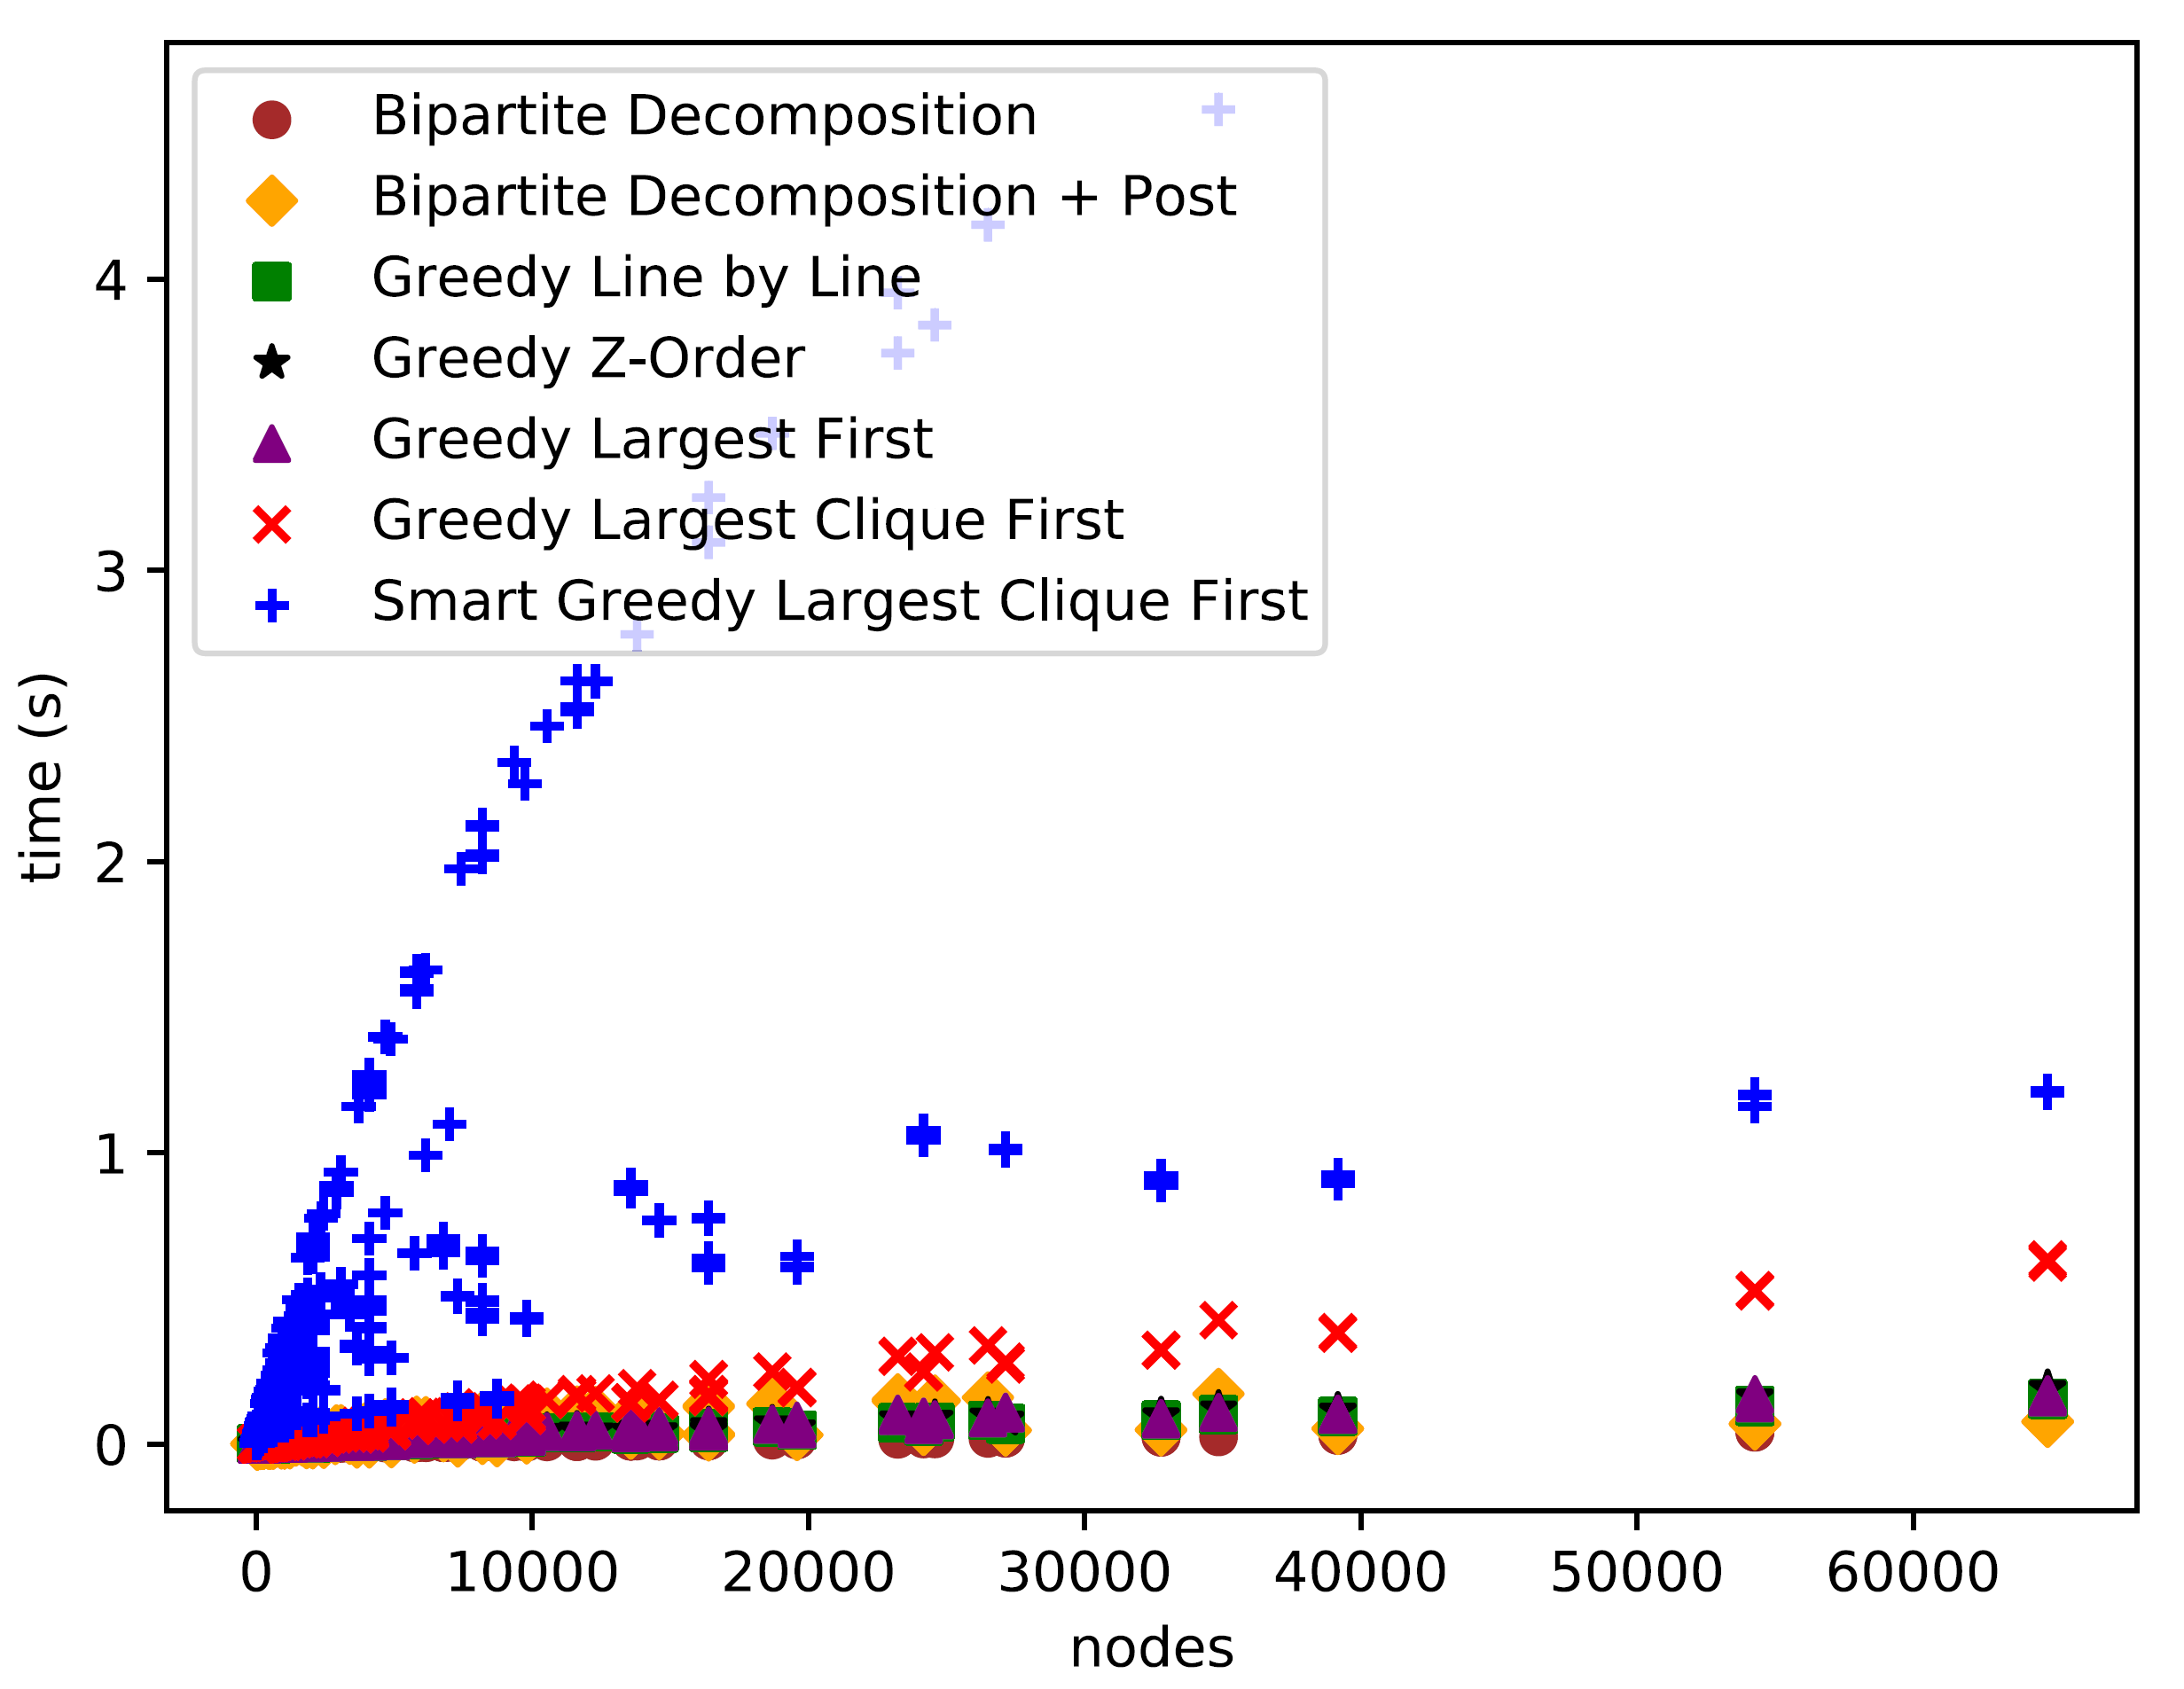
\includegraphics[width=\linewidth]{figures/time_results_2D.png}
      \caption{ET for coloring solution 2D}
    \end{subfigure}
    \hfill
    \begin{subfigure}{0.4\textwidth}
      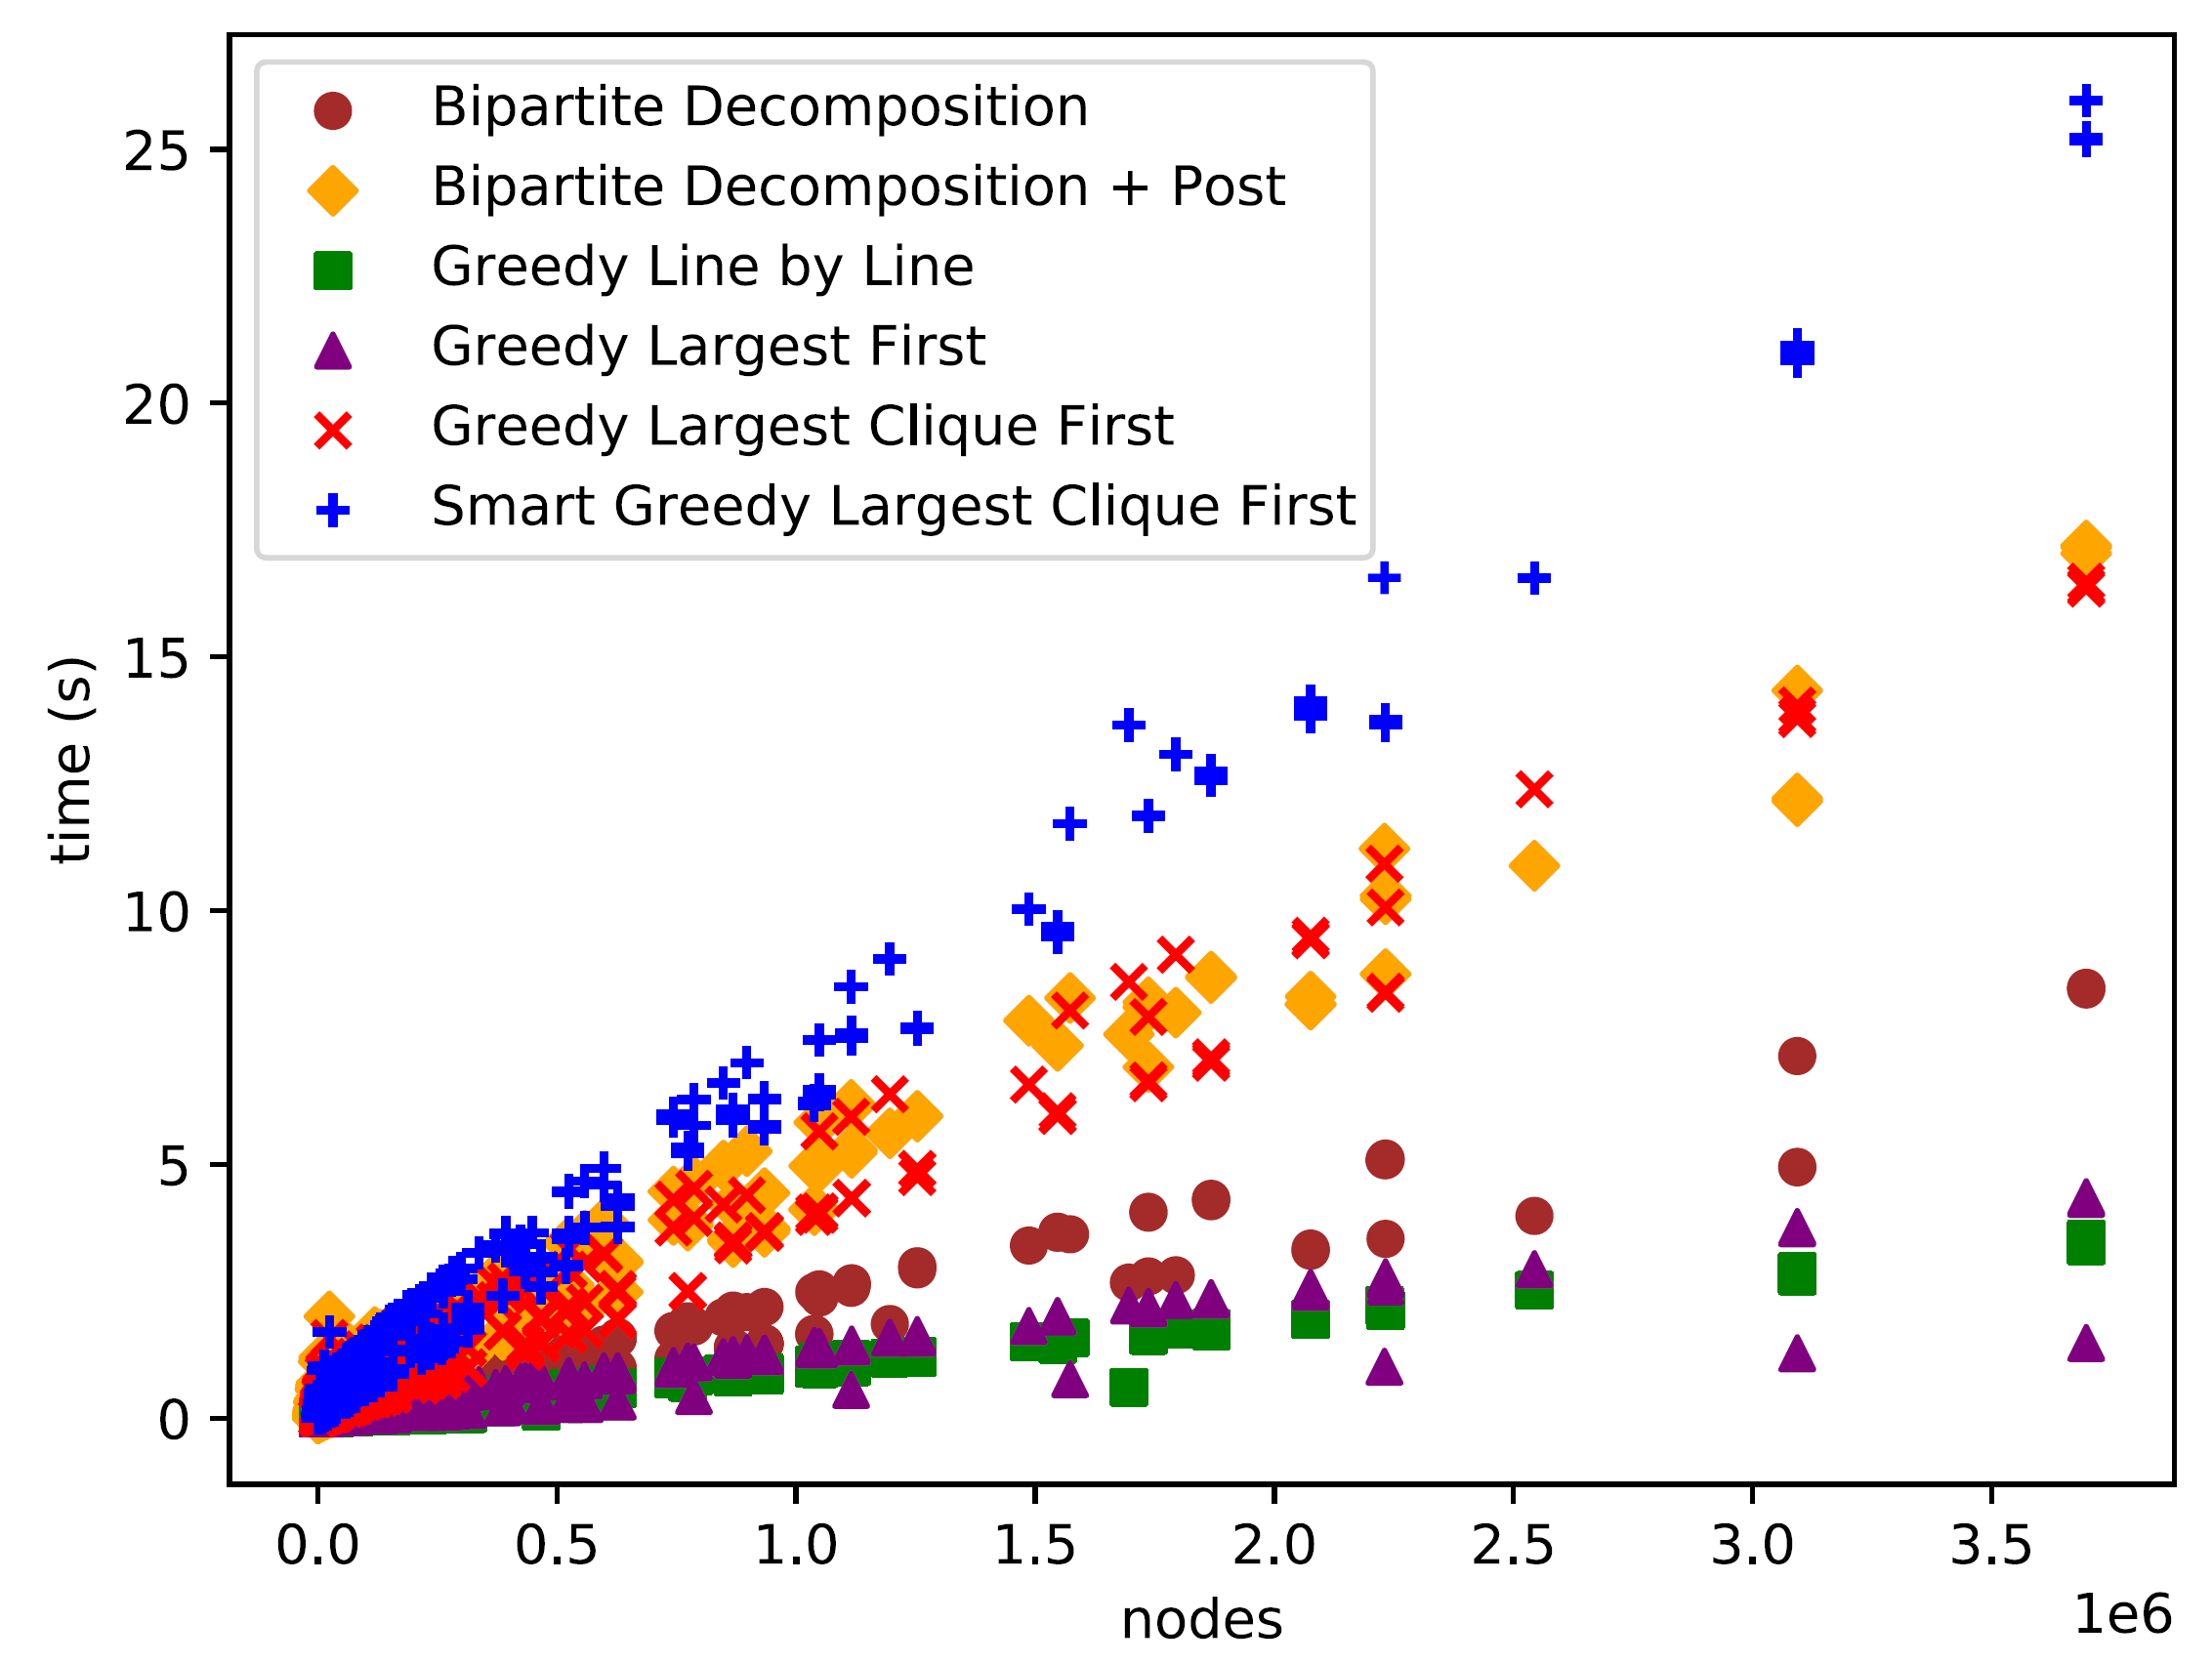
\includegraphics[width=\linewidth]{figures/time_results_3D.png}
      \caption{ET for coloring solution 2D}
    \end{subfigure}
  \end{figure}

  \footnotetext[1]{\scriptsize e.g. $\tau = 2$ and $\mathrm{prop} = 0.8$ means algo is within twice the 
  best-known for 80\%.}
\end{frame}